Een voeding van een PC heeft als ingangsspanning 230 Vac en als uitgangsspanning 12, 5, en 3,3 Vdc. De ingangsspanning moet dus omgezet worden naar een gelijkspanning en hij moet omgezet worden van 230 V naar bijvoorbeeld 12 V. Het verlagen van de spanning is de taak van de transformator\index{Transformator}\index{Transformer}. De transformator werkt met de inkomende wisselspanning, dus de uitgaande spanning is bijvoorbeeld 23 Vac.

In de elektronica wordt een transformator weergegeven met het symbool dat je ziet weergegeven in \ref{symbool:transformator}

\begin{figure}[h]

\includegraphics[width=5cm]{transformator}
\centering
\caption{Symbool van een transformator}
\label{symbool:transformator}
\end{figure}

Een transformator bestaat uit twee spoelen die verbonden zijn door een metalen-kern. De kern geleidt het magnetische veld dat door de primaire spoel wordt opgewekt, zie figuur \ref{fig:transformator3D}.

\begin{figure}[h]
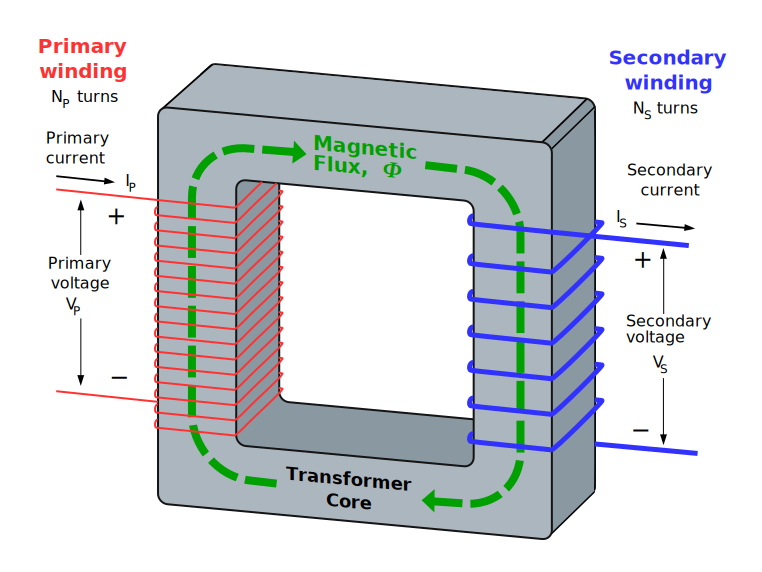
\includegraphics[width=10cm]{Transformer3d-col3}
\centering
\caption{Symbool van een 3D transformator}
\label{fig:transformator3D}
\end{figure}

Door het magnetische veld ontstaat in de tweede spoel een spanning en kan er stroom lopen door het circuit dat aan de tweede spoel gekoppeld zit. Als de primaire en de secundaire spoelen een gelijk aantal windingen hebben dan is de primaire spanning gelijk aan de secundaire spanning. Heeft de primaire spoel twee keer zoveel windingen als de secundaire spoel, dan wordt de spanning verlaagt met de helft. Dus 230 Vac aan de primaire kant wordt dan 115 Vac aan de secundaire kant. Heeft de primaire kant minder wikkelingen dan de secundaire kant dan wordt de spanning verhoogt.

De omrekening van primaire spanning naar secundaire spanning kan gedaan worden via de formule \[ V_s = V_p \frac{N_p}{N_s} \].
